\section{IMU随机误差模型及标定}

\begin{comment}
\end{comment}
\begin{frame}
\frametitle{IMU随机误差分类 \hfill 
\includegraphics[height=0.5cm]{00_logo.png}}
\begin{columns}
  \column{0.1\textwidth}
  
	\column{0.8\textwidth}
	\begin{enumerate}
		\item {\color{red}高斯白噪声} \quad		
		IMU数据连续时间上受到一个均值为0,方差为$\sigma$,各时刻之间相互独立的高斯过程$n(t)$:

\begin{equation}
  \begin{split}
    & E[n(t)] = 0 \\
    & E[n(t_1)n(t_2)] = \sigma^2 \delta(t1-t2)
  \end{split}
\end{equation}

其中,$\delta()$表示狄拉克函数.

	\item {\color{red}Bias随机游走}
	通常用维纳过程(wiener process)来建模bias随时间连续变化的过程,离散时间下称之为随机游走.

\begin{equation}
  \dot{b}(t) = n_b(t) = \sigma_b w(t)
\end{equation}

其中,$ w$是方差为1的白噪声.


\end{enumerate}
  
问题:实际上,IMU传感器产生的原始数据是连续的,而输出数据是离散的,离散和连续高斯白噪声存在何种关系?

  % \column{0.3\textwidth}
	% \begin{figure}[h]
	% 	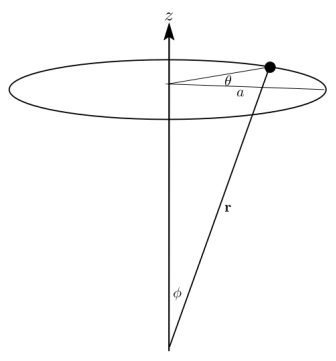
\includegraphics[trim=1.5 0 0 0, height=3.5cm,clip]{11_0.png}
	% 	% \caption{四个区域搜索空间}
  % \end{figure}
  
	\column{0.1\textwidth}

\end{columns}
\end{frame}

%%%%%%%%%%%%%%%%%%%%%%%%%%%%

\begin{frame}
  \frametitle{高斯白噪声的离散化 \hfill 
\includegraphics[height=0.5cm]{00_logo.png}}
  \begin{columns}
    \column{0.1\textwidth}
    
    \column{0.8\textwidth}

    只考虑高斯白噪声的积分
    \begin{equation}
      n_d[k] \triangleq n(t_0 + \Delta t) \simeq \frac{1}{\Delta t} \int ^{t_0+\Delta t}_{t_0} n(t) dt
    \end{equation}

    协方差为:
    \begin{equation}
      \begin{split}
        E(n^2_d[k]) &= E(\frac{1}{\Delta t^2} \int ^{t_0+\Delta t}_{t_0} \int ^{t_0+\Delta t}_{t_0} n(\tau) n(t))d\tau dt \\
        &= \frac{1}{\Delta t^2} \int ^{t_0+\Delta t}_{t_0} \int ^{t_0+\Delta t}_{t_0} E(n(\tau) n(t))d\tau dt \\
        &= \frac{\sigma^2}{\Delta t^2} \int ^{t_0+\Delta t}_{t_0} \int ^{t_0+\Delta t}_{t_0} \delta(t-\tau)d\tau dt \\
        &= \frac{\sigma^2}{\Delta t}        
      \end{split}
    \end{equation}
    
    \column{0.1\textwidth}
  
  \end{columns}
  \end{frame}   

%%%%%%%%%%%%%%%%%%%%%%%%%%%%

\begin{frame}
  \frametitle{高斯白噪声的离散化 \hfill 
\includegraphics[height=0.5cm]{00_logo.png}}
  \begin{columns}
    \column{0.1\textwidth}
    
    \column{0.8\textwidth}

    即:
    \begin{equation}
      n_d[k] = \sigma w[k]
    \end{equation}

    其中,
    \begin{equation}
      \begin{split}
        &w[k] \sim N(0, 1) \\
        &\sigma_d = \sigma \frac{1}{\Delta t}
      \end{split}
    \end{equation}
    
    也就是说高斯白噪声的连续时间表示到离散时间表示相差一个$\frac{1}{\Delta t}$,$\sqrt{\Delta t}$是传感器的采样时间.

    \column{0.1\textwidth}
  
  \end{columns}
  \end{frame}   

%%%%%%%%%%%%%%%%%%%%%%%%%%%%

\begin{frame}
  \frametitle{bias随机游走的离散化 \hfill 
\includegraphics[height=0.5cm]{00_logo.png}}
  \begin{columns}
    \column{0.1\textwidth}
    
    \column{0.8\textwidth}

    

      提取bias积分部分

      \begin{equation}
        b(t_0+\Delta t) = b(t_0) + \int ^{t_0+\Delta t}_{t_0} n_b(t) dt  
      \end{equation}

      由此可得离散化下的bias协方差:
      \begin{equation}
        E\{b^2(t_0+\Delta t)\} = E\{[b(t_0)+\int ^{t_0+\Delta t}_{t_0}n_b(t)dt][b(t_0)+\int ^{t_0+\Delta t}_{t_0}n_b(\tau)d\tau]\}  
      \end{equation}

      由于$E\{n_b(t)n_b(\tau)\} = \sigma^2_b \delta(t-\tau)$有:
      \begin{equation}
        E\{b^2(t_0+\Delta t)\} = E\{b^2(t_0)\} + \sigma^2_b \Delta t
      \end{equation}
    
    \column{0.1\textwidth}
  
  \end{columns}
  \end{frame}     


  %%%%%%%%%%%%%%%%%%%%%%%%%%%%

\begin{frame}
  \frametitle{bias随机游走的离散化 \hfill 
\includegraphics[height=0.5cm]{00_logo.png}}
  \begin{columns}
    \column{0.1\textwidth}
    
    \column{0.8\textwidth}

    即:
\begin{equation}
  b_d[k] = b_d[k-1] + \sigma_{bd}w[k]
\end{equation}

其中,
\begin{equation}
  \begin{split}
    & w[k] \sim N(0, 1)\\
    & \sigma_{bd} = \sigma_b \sqrt{\Delta t}
  \end{split}
\end{equation}

  bias随机游走的噪声方差从连续时间到离散之间需要乘以$\sqrt{\Delta t}$
    
    \column{0.1\textwidth}
  
  \end{columns}
  \end{frame}    

  %%%%%%%%%%%%%%%%%%%%%%%%%%%%

\begin{frame}
  \frametitle{高斯白噪声的离散化 \hfill 
\includegraphics[height=0.5cm]{00_logo.png}}
  \begin{columns}
    \column{0.1\textwidth}
    
    \column{0.8\textwidth}

    只考虑高斯白噪声的积分
    \begin{equation}
      n_d[k] \triangleq n(t_0 + \Delta t) \simeq \frac{1}{\Delta t} \int ^{t_0+\Delta t}_{t_0} n(t) dt
    \end{equation}

    协方差为:
    \begin{equation}
      \begin{split}
        E(n^2_d[k]) &= E(\frac{1}{\Delta t^2} \int ^{t_0+\Delta t}_{t_0} \int ^{t_0+\Delta t}_{t_0} n(\tau) n(t))d\tau dt \\
        &= \frac{1}{\Delta t^2} \int ^{t_0+\Delta t}_{t_0} \int ^{t_0+\Delta t}_{t_0} E(n(\tau) n(t))d\tau dt \\
        &= \frac{\sigma^2}{\Delta t^2} \int ^{t_0+\Delta t}_{t_0} \int ^{t_0+\Delta t}_{t_0} \delta(t-\tau)d\tau dt \\
        &= \frac{\sigma^2}{\Delta t}        
      \end{split}
    \end{equation}
    
    \column{0.1\textwidth}
  
  \end{columns}
  \end{frame}    


 